% !TEX root = thesis_draft.tex

\section{General Methods}

\subsection{Data set}
The EEG hyperscanning data used for this study was collected by
\textcite{newman_effects_2021} using two daisy-chained BioSemi ActiveTwo EEG
systems. Electrodes were placed according to the international 10–20 system.
Additionally, four electrodes were placed surrounding the eyes to monitor eye
movements and two were placed on the mastoids to serve as linked reference
electrodes. The technical details of the EEG hyperscanning setup were as
described by \textcite{barraza_implementing_2019}. Data was collected for 42
sessions, but 38 of those are analyzed here as during four sessions recording
issues were encountered.

\subsection{EEG pre-processing}

For each of the participants in the dyads, data was re-referenced to the average
of the mastoid electrodes and band-pass filtered to remove parts of the signals
with a frequency lower than 0.1 Hz and higher than 50 Hz. To prevent edge
artifacts one minute of padding consisting of mirrored data was added for the
duration of the filtering process. Next, the recorded data was split up into
trials which start one second before and end 1.5 seconds after stimulus
presentation. The pre-stimulus period was used for baseline correction. At this
stage, any linear trends were also removed for each trial. This removed slow
low-frequency drifts from the data, which can otherwise show up as artifacts
during frequency analysis \parencite{schoffelen_why_2010}.

\begin{table}[!htpb]
  \caption{Trial counts after pre-processing and how often they occur. For most sessions, a maximum of 10 trials were removed. The outlier of 84 trials is session 25.}
  \label{tab:trial_counts}
  \begin{tabular}{r | r r r r r r r r r r}
    \hline
    trial count (1) & 84  & 144 & 152 & 157 & 163 & 164 & 165 & 166 & 169 & 170\\
    frequency (1)   & 1   & 1   & 1   & 1   & 1   & 1   & 1   & 1   & 1   & 2  \\\hline
    trial count (2) & 171 & 172 & 173 & 174 & 175 & 177 & 178 & 179 & 180      \\
    frequency (2)   & 1   & 3   & 1   & 4   & 4   & 1   & 2   & 3   & 8        \\\hline
  \end{tabular}
\end{table}

Each recorded trial was manually inspected. When electrodes did not make a good
connection to the skin or otherwise regularly produced unusable data, they were
removed from the data set and reconstructed using spline interpolation from
neighbouring electrodes. If an electrode drifted or was very noisy for only one
or a few trials, it was interpolated in these trials only. If too many
neighbouring electrodes were affected, interpolation became impossible and
instead the whole trial was rejected. Trials were also rejected when they
contained more than four electrode signals that required interpolation. See for
how many trials remained Table~\ref{tab:trial_counts}. Eye blinks, muscle
activity and other localized artifacts were left alone at this stage. Instead,
they were handled by subtracting highly localized and artifactual components
from the data as obtained using independent component analysis (ICA).

\begin{figure}[!htpb]
  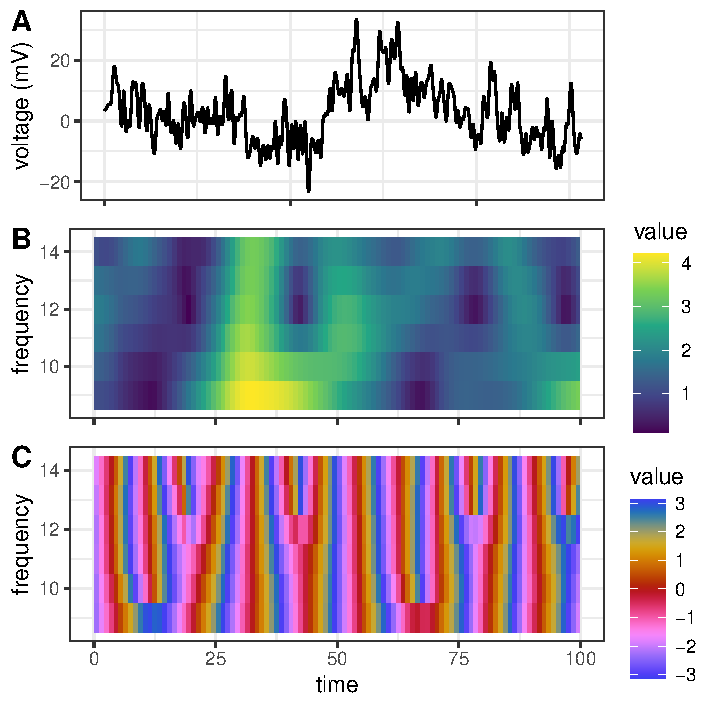
\includegraphics[width=\linewidth]{../stats/results/freqdomain.pdf}
  \caption{Time-frequency plot showing (B) amplitude and (C) phase values. Example frequency domain representation of session 2, participant 1, trial 1, Pz electrode, alpha band (9--14 Hz). The raw data used for the frequency analysis of this trial is shown in (A).}
  \label{fig:freqanalysis}
\end{figure}

\subsection{Time-frequency analysis}
The first step to calculating the phase locking value (PLV), circular
correlation (CCorr) and imaginary part of coherency (ImagCoh) measures consists
of transforming the data into the frequency domain. We do so once every 10
milliseconds for both the alpha band (9--14 Hz) and theta band (4--7 Hz). For
most of the analysis, we use a Hann taper with a frequency dependent window
length of four cycles per window. At least four cycles are recommended by
\textcite{ayrolles_hypyp_2021}. For the lowest frequency of interest (4 Hz),
this results in a window of exactly one second. As a result, the amplitude and
phase of a signal can only be estimated for moments during the trial where half
a second of extra data is available before and after. Because of that, we narrow
the duration of a trial for the purposes of inter-brain synchrony (IBS)
calculation from zero to one second after stimulus presentation exactly.

The result of the frequency analysis is a complex valued Fourier spectrum $x_i$
for each combination of participant, electrode and frequency in the frequency
band. From this spectrum, the amplitudes $r_i$ and phases $\phi_i$ of the input
signal can be extracted by representing the complex values in polar
coordinates. See Figure~\ref{fig:freqanalysis} for a visualization of $r_i$ and
$\phi_i$ of an example signal.

\subsection{Measure definitions}

We compare the signals of homologous electrodes between participants, e.g. we
only compare the signal of the Fz electrode of participant 1 with participant
2's Fz electrode, not with other electrodes. While it is technically possible
to do otherwise, we would lose the ability to conveniently interpret high IBS
as suggestive of similar mental processes in both participants.

The PLV measures whether the difference in the phase of two signals is kept
constant. The PLV measure is defined by \textcite{lachaux_measuring_1999} as
\begin{equation}\label{eq:plv}
\text{PLV} = \cfrac{1}{T}\left|\sum_{t=1}^T e^{i(\phi_i - \phi_j}\right|,
\end{equation}
where $\phi_i$ and $\phi_j$ are the phases of input frequency spectra $x_i$ and
$x_j$ of the different participants. As you can see, the PLV measure is
calculated by averaging along a dimension of size $T$. For this
analysis, we will be averaging over time resulting in one measurement per trial
and frequency. It is also possible to calculate PLV and the other measures
discussed in the current study over trials instead, resulting in a measure of
within-trial IBS. But within the context of \textcite{newman_effects_2021}'s
experiment, how IBS develops over trials is much more interesting. (See
Appendix~\ref{app:task} for more information about
\textcite{newman_effects_2021}'s task.)

While we calculate measures (including PLV) for each whole number frequency
within the frequency band of interest, we are not interested in their
differences within the same band. Instead, we average these values resulting
in a single measure per trial and frequency band. This should contribute to a
more stable estimate. Our PLV implementation was validated against Fieldtrip's
implementation.

\begin{figure}[!htpb]
  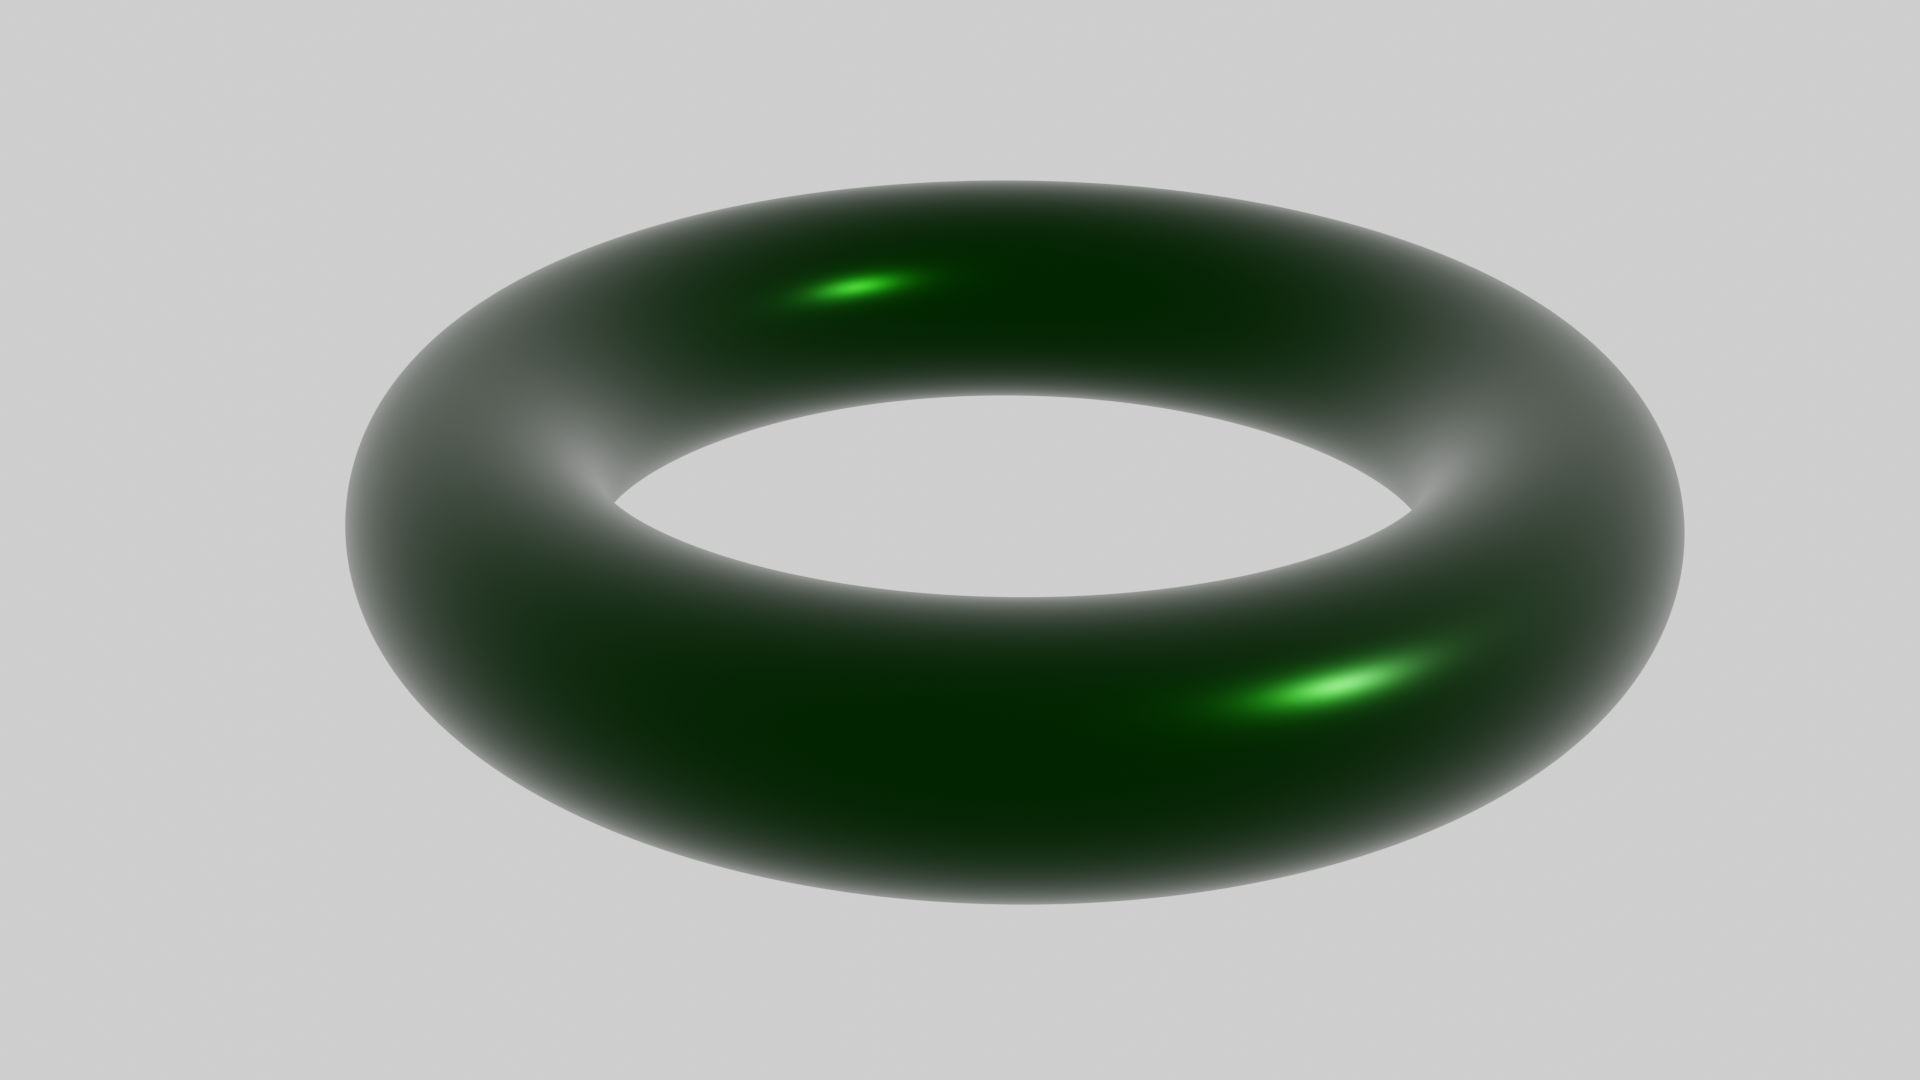
\includegraphics[width=\linewidth]{torus.png}
  \caption{A torus. Bivariate circular data can be thought of as points on a torus. Rendered using Blender \parencite{blender_online_community_blender_2022}.}
  \label{fig:torus}
\end{figure}

CCorr is an analogue of Pearson correlation for angular values
like a phase. It seems to have been first derived by
\textcite{fisher_correlation_1983}, but most recent implementations are based on
the definition by \textcite{jammalamadaka_correlation_1988} which has more
recently been republished in a book \parencite{jammalamadaka_topics_2001}:
\begin{equation}\label{eq:ccorr}
\text{CCorr} = \cfrac{\sum_{t = 1}^T \sin\left(\phi_i - \bar{\phi_i}\right) \sin\left(\phi_j - \bar{\phi_j}\right)}
                {\sqrt{\sum_{t = 1}^T \sin^2\left(\phi_i - \bar{\phi_i}\right) \sin^2\left(\phi_j - \bar{\phi_j}\right)}}.
\end{equation}
Within this equation, $\bar{\phi_i}$ is the circular mean which can be
defined as
\begin{equation}
\bar{\phi_i} = \operatorname{arg} \sum_{t=1}^T e^{\phi_ti},
\end{equation}
where `$\operatorname{arg}$' gives us the angle we get when converting the sum
to polar form. When interpreting normal Pearson correlation coefficients, I
often imagine plotting the two variables of interest against each other. The
coefficient then tells us how close the data points are to lying on a line. With
CCorr values, it is possible to do the same, but instead of a normal
plot you should imagine the data points existing on a torus
\parencite[see also Figure~\ref{fig:torus}]{lee_circular_2010}. Our
implementation of the CCorr measure was inspired by and validated against
the implementation in the CircStat MATLAB toolbox
\parencite{berens_circstat_2009}.

Finally, the ImagCoh measure looks not just at the phase of signals
but also takes into account the amplitude. It is defined by
\textcite{nolte_identifying_2004} as
\begin{equation}\label{eq:imagcoh}
\text{ImagCoh} = \operatorname{Im}\left(\cfrac{S_{ij}}{\sqrt{S_{ii}S_{jj}}}\right),
\end{equation}
where $S_{ij}$ is the crossspectral density of the signals and $S_{ii}$ and
$S_{jj}$ are the autospectral densities of each of the signals. These spectral
densities are estimated directly from the Fourier transformed data $x_i$ and
$x_j$.
\begin{equation}
S_{ij} = \cfrac{1}{T} \sum_{t = 1}^{T} x_i {x_j}^\ast \text{ \parencite{schoffelen_what_2011}},
\end{equation}
where ${x_j}^\ast$ is the complex conjugate of $x_j$. Our implementation of the
ImagCoh measure was validated against Fieldtrip's.

\subsubsection{Statistics}

We use linear mixed effect models with random intercepts over sessions and
electrodes. More complex random effect structures are not supported by the data,
and in some cases including a random intercept for electrodes is not either when
the data is too homogeneous across electrodes. In that case, said random
intercept is left out. Next to any fixed effects of interest, fixed effects of
working memory load, trial and stimulus type were included if they significantly
contributed to the model to account for possibly confounding effects of those.
The models underlying the model comparisons referred to in the text are
reproduced in Appendix~\ref{app:lme}.

\subsection{Software}

All manipulations of the EEG data were performed with Fieldtrip version
20211102 \parencite{oostenveld_fieldtrip_2011} running on MATLAB R2020b. All
IBS measures were implemented from scratch in both MATLAB for use in the
empirical study and R 4.2.0 \parencite{r_core_team_r_2022} for use in the
simulation study. Graphs were generated in R using tidyverse 1.3.2
\parencite{wickham_welcome_2019}, eegUtils 0.7.0
\parencite{craddock_eegutils_2022}, gganimate 1.0.7
\parencite{pedersen_gganimate_2020}, ggh4x 0.2.3
\parencite{van_den_brand_ggh4x_2022}, ggpubr 0.4.0
\parencite{kassambara_ggpubr_2020}, ggvoronoi 0.8.5
\parencite{garrett_ggvoronoi_2022} and pals 1.7 \parencite{wright_pals_2021}.
All statistical tests were performed using R as well, using lme4 1.1.29
\parencite{bates_fitting_2015} for the linear mixed effect models. For the
generalized additive mixed effect models mgcv 1.8.41
\parencite{wood_generalized_2006} was used alongside itsadug 2.4
\parencite{van_rij_itsadug_2020} for plotting those models. To generate
simulated correlated data, faux 1.1.0 \parencite{debruine_faux_2021} was used.
Finally, Python 3.10.8 \parencite{python_software_foundation_python_2021} was
used to train and evaluate classifiers, along with imbalanced-learn 0.1.9
\parencite{lemaitre_imbalanced-learn_2017}, NumPy 1.23.3
\parencite{harris_array_2020}, pandas 1.5.0 \parencite{mckinney_data_2010},
scikit-learn 1.1.2 \parencite{pedregosa_scikit-learn_2011} and SciPy 1.9.1
\parencite{virtanen_scipy_2020}.

Parts of the R and MATLAB code used in this study are available at TODO.
